\chapter{Ain’tea: managing data uncertainty at the language level}
\label{chapt:aintea}
\chapterPage{
After identifying and discussing the key concepts associated with data uncertainty, this chapter presents \langName{}, a language that integrates them directly into the grammar, type system and semantics part. 
To validate and exemplify our approach, we apply it to a smart-grid scenario and compare it to framework-based approaches.
We show that developers benefit from the language semantics and type system which guide them to manipulate uncertain data without deep probability theory knowledge.}

\section{Introduction}

%% Research questions
\paragraph{Delayed actions}
General research question:
\begin{center}
	\textbf{RQ1}: Do current state of the art solutions allow modeling and reasoning over delayed actions?  
\end{center}

Sub research questions:
\begin{itemize}
	\item \textbf{RQ1.1}: How current approaches model the evolution of the context and/or the evolution of the behavior of systems over time?
	\item \textbf{RQ1.2}: Do these solutions model actions, their circumstances and their effects?
	\item \textbf{RQ1.3}: What are the solutions that enable the reasoning over the evolving context and/or behavior of systems?
\end{itemize}


\paragraph{Uncertainty}

%% Methodology
Snowballing approach~\cite{DBLP:conf/ease/Wohlin14}

\paragraph{Inclusion criteria}
\begin{itemize}
	\item \textbf{IC1}: The paper has been published before the May 31 2019
	\item \textbf{IC2}: The paper is available online and written in English
	\item \textbf{IC3}: The paper describes a modeling approach that abstract the context or behavior of a system.
	\item \textbf{IC4}: The paper describes an approach that enables to reason or navigate through a temporal model.
\end{itemize}

\paragraph{Exclusion criteria}
\begin{itemize}
	\item \textbf{EC1}: The paper has less than 4 pages (short paper).
	\item \textbf{EC2}: The paper presents a work in progress (workshop papers), a poster, vision or doctoral studies.
	\item \textbf{EC3}: The paper describes a secondary study (\eg literature reviews, lessons learned).
	\item \textbf{EC4}: The document has not been published in a venue with a peer-review process. For example, technical and research report or white papers.
	\item \textbf{EC5}: The document is an introduction to the proceedings of a venue or a special issue.
\end{itemize}

However, the references of papers rejected are considered for the snowballing iteration.
\section[Data uncertainty]{\gls{duc}}
\label{sec:example:duc}

\subsection{Impacts of ignoring data uncertainty} 
\label{subsec:example-possible-consequences}
%Although power grids are becoming more and more automated, today human interventions are still the norm.
%For example, most fuses inside cabinets or substations are manually modified by technicians rather than automatically reconfigured.
%As a consequence, the states of fuses are manually documented by technicians on the field. 
%This of course results in mistakes. 
%One way to address this problem is to take uncertainty into consideration.
%This means considering fuse states as uncertain.
%
%As a consequence, this uncertainty propagates to the load calculation formulas, which depend on the fuse states.
%We call this type of uncertainty \textit{uncertain discrete number}. 
%It also propagates to the final load.
%We refer to these values as \textit{uncertain continuous numbers}. 
%In other words, if the uncertainty of fuse states is not considered, it exists a non-null probability that the observed phenomenon does not reflect the real situation.
%Cable load approximations are used to detect cable overloads and to reconfigure the network if necessary.
%By not considering uncertainty, wrong reconfigurations might be triggered, which could be even worse than if no change would have been applied.
%
%In order to model the electricity flow, we can first use a structure or a class to abstract entities (meter, substation, etc.).
%Then, it can be abstracted by linking different entities.
%For example, the substation in Figure~\ref{fig:intro-schema-topology1} contains two references to the cabinet.
%These references are uncertain due to the uncertain nature of fuse states.
%We refer to these references as \textit{uncertain references}.

Although power grids are becoming more and more automated, today human interventions are still the norm.
For example, most fuses are manually modified by technicians rather than automatically reconfigured.
The states of fuses are thus manually documented by technicians on the field. 
This of course results in mistakes. 
One way to address this problem is to take uncertainty into consideration.
This means considering fuse states as uncertain.

As a consequence, this uncertainty propagates to the load calculation formulas, which depend on the fuse states.
If the uncertainty of fuse states is not considered, it exists a non-null probability that the observed phenomenon does not reflect the real situation.
For example, as we have seen in the previous subsection, a modification of the electricity flow may impact the load of a cable with a factor of 2.
Cable load approximations are used to detect cable overloads and to reconfigure the network if necessary.
By not considering uncertainty, wrong reconfigurations might be triggered, which could worsen the situation.

\subsection{Managing uncertainty is not effortless}
In the following, we describe how uncertainty is commonly handled by application developers using current state-of-the-art approaches. 
We show, through code samples, the limitations of these approaches and why we think that these limitations can be addressed by integrating uncertainty management directly at the language level.
In the code excerpts below, we compute the average cable load over the whole grid based on uncertain cable loads. 
A complete version can be found on the GitHub repository. 
All codes contain at least two classes: \textit{SmartGrid} and \textit{Cable}.
The former contains two fields: an array of Cables named \textit{cables} and a function to compute the average load of cables, named \textit{compute\_avg\_load}.
The latter contains one field: an uncertain number which represents the uncertain load.

\paragraph{Manual implementation} 
%One approach for managing uncertainty is to manually implement all the required features.
%Listing~\ref{lst:example-from-scratch} illustrates this (in Python).
%The excerpt contains three classes, UNumber (lines 1--21), SmartGrid (lines 23--31), and Cable (lines 33--35).
%
%As we can see, this approach comes with several drawbacks.
%First, developers are required to have deep knowledge of probability theory.
%For example, uncertainty can be represented by a normal distribution identified by its mean and variance as shown in the constructor ($\_\_init\_\_$), lines 3 and 4.
%One needs knowledge on how to represent it, how to add two normal distributions, ...
%This type is used in the constructor of the class \textit{Cable} to initialize the cable load (line 28).
%In order to support uncertainty propagation through arithmetic operations, one can think of overloading existing arithmetic operations or defining new ones. 
%Languages like Python and C\# allow operator overloading.
%The method definitions $\_\_plus\_\_$ and $\_\_div\_\_$ overload the '+'  and '/' operations respectively. 
%These operators are later used in the SmartGrid class definition to compute the average load, lines 23 and 25.
%
%Second, manual implementation inevitably increases the size of the code base.
%This will de facto augment the risk of errors in the code.
%Plus, the code will be more difficult to maintain afterwards.
%
%Third, although some languages offer the possibility to overload operators, some typing errors can only be detected at runtime. 
%For instance, since Python is dynamically typed, performing an addition operation between \textit{UNumber} and an \textit{UBoolean} fails and raises an exception only at runtime.
%Whilst, statically typed languages such as C\# can detect such typing errors at development time. 
%Nonetheless, the returned exception message would not be particularly meaningful, as can be seen on the example of  C\#: \textit{Operator `+' cannot be applied to operands of type UNumber and UBoolean}. 
%Handling uncertainty at the language-level and extending the typing system, would significantly improve developers' experience and make it possible to detect typing errors at early stages.

One approach for managing uncertainty is to manually implement all the required features.
Listing~\ref{lst:example-from-scratch} illustrates this in Python.
In addition to the \textit{SmartGrid} and \textit{Cable} class, the excerpt contains an additional one: \textit{UNumber}.

As we can see, this approach comes with several drawbacks.
First, developers are required to have deep knowledge of probability theory.
For example, uncertainty can be represented by a normal distribution identified by its mean and variance as shown in the constructor (\textit{\_\_init\_\_}), line 2.
One needs knowledge on how to represent it, how to add two normal distributions, etc.
For example, here we overload the sum and the division operators for two normal distributions (\textit{\_\_plus\_\_} and \textit{\_\_div\_\_} methods).

Second, manual implementation inevitably increases the size of the code base.
This will de facto augment the risk of errors in the code.
Plus, the code will be more difficult to maintain afterwards.

Third, although some languages offer the possibility to overload operators, some typing errors can only be detected at runtime. 
For instance, since Python is dynamically typed, performing an addition operation between two types of uncertain numbers (\ie represented by two classes) fails and raises an exception only at runtime.
Whilst, statically typed languages such as C\# can detect such typing errors at development time. 
Nonetheless, the returned exception message would not be particularly meaningful, as can be seen on the example of  C\#: \textit{Operator `+' cannot be applied to operands of type UNumber1 and UNumber2}.

%\begin{lstlisting}[style=pythonStyle, caption=Manual management of uncertainty in Python, label=lst:example-from-scratch, linewidth=0.97\textwidth
%]
%class UNumber:
%    def __init__(self, mean=0, variance=0):
%        [...]
%
%    def __add__(self, other):
%       [...] # typing error management + casting other to UNumber if it is a Number
%       return UNumber(self.mean + other.mean, self.variance + other.variance)
%
%    def __div__(self, other):
%       [...] # typing error management + casting other to UNumber if it is a Number
%       value = ((self.mean / other.mean) + 
%             (self.mean * other.variance)) / pow(other.mean, 3)
%       variance = (self.variance / other.mean) +
%             (pow(self.mean, 2) * other.variance) / pow(other.mean, 4)
%       return UNumber(value, variance)
%
%class SmartGrid:
%    def __init__(self):
%        self.cables = []
%
%    def compute_avg_load(self):
%        sum_load = 0
%        for c in self.cables:
%            sum_load += c.load
%        return sum_load / len(self.cables)
%
%class Cable:
%    def __init__(self, id, load=UNumber(0, 0)):
%       [...]
%\end{lstlisting}

\begin{lstlisting}[style=pythonStyle, caption=Manual management of uncertainty in Python, label=lst:example-from-scratch, linewidth=0.97\textwidth
]
class UNumber:
  def __init__(self, mean=0, variance=0):
    [...]
    
  def __add__(self, other):
    [...] # typing error management + casting other to UNumber if it is a Number
    return UNumber(self.mean + other.mean, self.variance + other.variance)
    
  def __div__(self, other):
    [...] # typing error management + casting other to UNumber if it is a Number
    value = ((self.mean/other.mean) + (self.mean*other.variance)) / pow(other.mean, 3)
    variance = (self.variance / other.mean) +
             (pow(self.mean, 2) * other.variance) / pow(other.mean, 4)
    return UNumber(value, variance)

class SmartGrid:
  [...]
  def compute_avg_load(self):
    sum_load = 0
    for c in self.cables:
      sum_load += c.load
    return sum_load / len(self.cables)
    
class Cable:
  def __init__(self, id, load=UNumber(0, 0)):
    [...]
\end{lstlisting}

\paragraph{Using existing libraries for probability theory}
%Since uncertainty management relies on probability theory, another approach is using a library implementing common probability distributions.
%%\footnote{\url{https://docs.scipy.org/doc/scipy/reference/stats.html}}
%Staying in Python, there is a widely used library called SciPy library\footnote{\url{https://www.scipy.org/}} and in particular the \textit{stats} module, defining different probability distributions, e.g. the Bernoulli and the Gaussian distributions (cf. Section~\ref{sec:data-uncertainty}).
%Whereas these libraries are suitable to compute different properties of probability distributions, it remains the responsibility of developers to define how to perform arithmetic operations on distributions.
%Listing~\ref{lst:limit-lib-proba} shows an example of the definition of the\textit{ add\_gaussian} method, responsible for adding up two uncertain numbers represented as Gaussian distributions. 
%
%Using such libraries does not prevent developers to have a deep understanding of the probability theory.
%They have been designed to help them manipulating probability distributions, but they still required knowledge about them.
%For example, as shown in Listing~\ref{lst:limit-lib-proba}, one may access the mean and the variance of a normal distribution.
%However, she or he needs to know how two normal distributions can be added.
%This also increases the code base and thus is prone to errors.
%Finally, as it is a library, typing errors will still remain either detected at runtime or not helpful for developers.
Since uncertainty management relies on probability theory, another approach is using a library implementing common probability distributions.
%\footnote{\url{https://docs.scipy.org/doc/scipy/reference/stats.html}}
Staying in Python, there is a widely used library called SciPy\footnote{\url{https://www.scipy.org/}} and in particular the \textit{stats} module, defining different probability distributions.
Whereas these libraries are suitable to compute different properties of probability distributions, it remains the responsibility of developers to define how to perform arithmetic operations on distributions, as depicted in \autoref{lst:limit-lib-proba}.

Using such libraries does not prevent developers to have a deep understanding of the probability theory.
They have been designed to help them manipulating probability distributions, but they still required knowledge about them.
For example, as shown in Listing~\ref{lst:limit-lib-proba}, one may access the mean and the variance of a normal distribution.
However, she or he needs to know how two normal distributions can be added.
This also increases the code base and thus is prone to errors.
Finally, as it is a library, typing errors will still remain either detected at runtime or not helpful for developers.


%\begin{lstlisting}[style=pythonStyle, caption=Limitation using a probability library (Python), label=lst:limit-lib-proba, linewidth=0.97\textwidth]
%from scipy.stats import norm
%
%def add_gaussian(g1, g2):
%    [...]
%    return norm(g1.mean() + g2.mean(), g1.var() + g2.var())
%
%def div_gaussian(g1, g2):
%   [...]
%
%class SmartGrid:
%    def __init__(self):
%        self.cables = []
%
%    def compute_avg_load(self):
%        sum_load = 0
%        for c in self.cables:
%            sum_load = add_gaussian(sum_load, c.load)
%        return div_gaussian(sum_load, len(self.cables))
%
%class Cable:
%    def __init__(self, id, load=norm(0, 0)):
%        [...]
%\end{lstlisting}

\begin{lstlisting}[style=pythonStyle, caption=Limitation using a probability library (Python), label=lst:limit-lib-proba, linewidth=0.97\textwidth]
from scipy.stats import norm

def add_gaussian(g1, g2):
    [...]
    return norm(g1.mean() + g2.mean(), g1.var() + g2.var())

def div_gaussian(g1, g2):
   [...]

class SmartGrid:
    [...]
    def compute_avg_load(self):
        sum_load = 0
        for c in self.cables:
            sum_load = add_gaussian(sum_load, c.load)
        return div_gaussian(sum_load, len(self.cables))

class Cable:
    def __init__(self, id, load=norm(0, 0)):
        [...]
\end{lstlisting}

\paragraph{Using existing libraries for uncertainty}
%Another commonly used approach is to use existing libraries for data uncertainty.
%For example, in Python, using the \textit{uncertainties~\cite{url:uncertainties} library}, a developer can manipulate uncertain floats using variables of type \textit{ufloat}.
%The uncertainty propagation is handled transparently.
%In Listing~\ref{lst:example-python-uncertainties}, we depict a minimalistic excerpt of the necessary code to compute the mean load using an existing library for data uncertainty.
%Unlike the previous code snippet, this listing contains only two classes, SmartGrid and Cable.
%Moreover, the cable load property initialization uses \textit{ufloat} instead of \textit{UNumber}.
%
%Using a library can tackle the two first drawbacks existing in the previous approach: required knowledge of probability theory and code complexity.
%Indeed, the implementation of the probability theory is encapsulated inside the library.
%Developers will just use it through its API.
%The complexity of the implementation, with the possible errors, are also pushed to the complexity.
%We can argue that the library will be well tested and documented.
%
%However, similarly to the previous example, this approach does not extend the type system.
%If the language relies on a dynamic type system (like in Python), then typing errors are raised only at runtime.
%In any case, raised exceptions are not very meaningful.
%For example, if two distributions are sum whereas the operator has not been overloaded for the input distributions, then the error message will just state this operation is not implemented, without any more information.
Another commonly used approach is to use existing libraries for data uncertainty.
For example, in Python, using the \textit{uncertainties}~\cite{url:uncertainties} library, a developer can manipulate uncertain floats using variables of type \textit{ufloat}.
The uncertainty propagation is handled transparently.
In Listing~\ref{lst:example-python-uncertainties}, we depict the code of the load average computation using this library.
The only difference from the previous code snippet, is the missing of the \textit{UNumber} class, not required anymore, and the use of the \textit{ufloat} type for the cable load variable.

Using a library can tackle the two first drawbacks existing in the previous approach: required knowledge of probability theory and code complexity.
Indeed, the implementation of the probability theory and its complexity are encapsulated inside the library.
We can argue that the library will be well tested and documented.
However, similarly to the previous example, this approach does not extend the type system.\looseness-1
%If the language relies on a dynamic type system (like in Python), then typing errors are raised only at runtime.
%In any case, raised exceptions are not very meaningful.
%For example, if two distributions are sum whereas the operator has not been overloaded for the input distributions, then the error message will just state this operation is not implemented, without any more information.

%\begin{lstlisting}[style=pythonStyle, caption=Managing uncertainty in Python using uncertainties~\cite{url:uncertainties}, label=lst:example-python-uncertainties, linewidth=0.97\textwidth, escapechar=\%]
%from uncertainties import ufloat
%
%class SmartGrid:
%    def __init__(self):
%        self.cables = []
%
%    def compute_avg_load(self):
%        [...] # same as in %\autoref{lst:example-from-scratch}%
%
%class Cable:
%    def __init__(self, p_id, p_load=ufloat(0, 0)):
%        self.id = p_id
%        self.load = p_load
%\end{lstlisting}
\begin{lstlisting}[style=pythonStyle, caption=Managing uncertainty in Python using uncertainties~\cite{url:uncertainties}, label=lst:example-python-uncertainties, linewidth=0.97\textwidth, escapechar=\%]
from uncertainties import ufloat

class SmartGrid:
  def __init__(self):
    self.cables = []

  def compute_avg_load(self):
    [...] # same as in %\autoref{lst:example-from-scratch}%

class Cable:
  def __init__(self, id, load=ufloat(0, 0)):
    [...]
\end{lstlisting}

\paragraph{Using a probability programming framework}
Developers can also use a probabilistic programming framework like Infer.NET~\cite{url:InferNET18} or PyMC3~\cite{DBLP:journals/peerj-cs/SalvatierWF16}.
These frameworks allow defining complex probabilistic models and applying inference algorithms.
Contrary to previously described libraries, these frameworks put an effort to set a proper API.
They can be thought as internal domain-specific languages (DSL)\cite{fowler2010domain}\footnote{Martin Fowler defines a DSL as \textquote{a computer programming language of limited expressiveness focused on a particular domain}\cite{fowler2010domain}. An internal DSL is defined inside a general-purpose language, using only a subset of its concept.}.
In Listing~\ref{lst:limit-proba-prog-fw}, we show how the cable load can be computed using the Infer.NET framework.
This approach exposes probability as a first-class language citizen. 
Hence, developers are expected to manipulate probability distributions and not uncertain data types. 
This framework relies on an inference engine to transparently combine probability distributions.
Using such an approach requires a decent acquaintance with probability theory.
We can assume that they are heavily tested, which limits the number of errors.
Plus, in this framework they map arithmetic operators to the combination of probability distributions: developers do not require to create additional work as with the library approach.
But, as it is not implemented at the language level, the typing system is not extended.
Errors will thus either be raised at runtime or not be helpful for developers.

\begin{lstlisting}[style=cSharpStyle, caption=Limitation using a probability programing framework (C\#), label=lst:limit-proba-prog-fw, linewidth=0.97\textwidth]
public class SmartGit {
  public List<Cable> cables { get; private set; }
  private readonly InferenceEngine inference;

  public Gaussian computeAvgLoad() {
    Variable<double> sum = Variable.GaussianFromMeanAndVariance(0,0).Named("sum");
    int i = 0;
    foreach(Cable c in cables)
      sum = (sum + c.load).Named("sum" + i);
      i++;
    Variable<double> result = (sum / cables.Capacity).Named("AvgLoad");
    return (Gaussian) this.inference.Infer(result);
  }
}

public class Cable {
  public Variable<double> load { get; set; }
}
\end{lstlisting}

\paragraph{Sum-up}
Using state-of-art solutions to manage uncertainty, developers have three possibilities: manual implementation, using existing libraries or using a probability programming framework.
As detailed in this section, these approaches will cope with at least one of these drawbacks: developers require a deep understanding of the probability theory, code base will increases which augments the risk of errors, and the type systems may detect errors at runtime or do not provide helpful messages.

%By enhancing uncertainty management as a first-class language citizen, we cope with these three disadvantages.
%In Figure~\ref{fig:motivation-aintea-overview}, we give an overview of our language, \languageName{}.
%Using our contribution, developers can instantiate uncertain variables (boo-lean, numeric or reference) and combine them using the same operators as they are used to (arithmetic, boolean, comparison).
%Plus, we also define new operators to reason over the uncertainty, or the confidence level, of manipulated variables.
%Finally, the type system will be able to detect errors related to probability distribution manipulation, at compilation time as we choose a static type system, with helpful messages.

%\begin{figure}
%	\centering
%	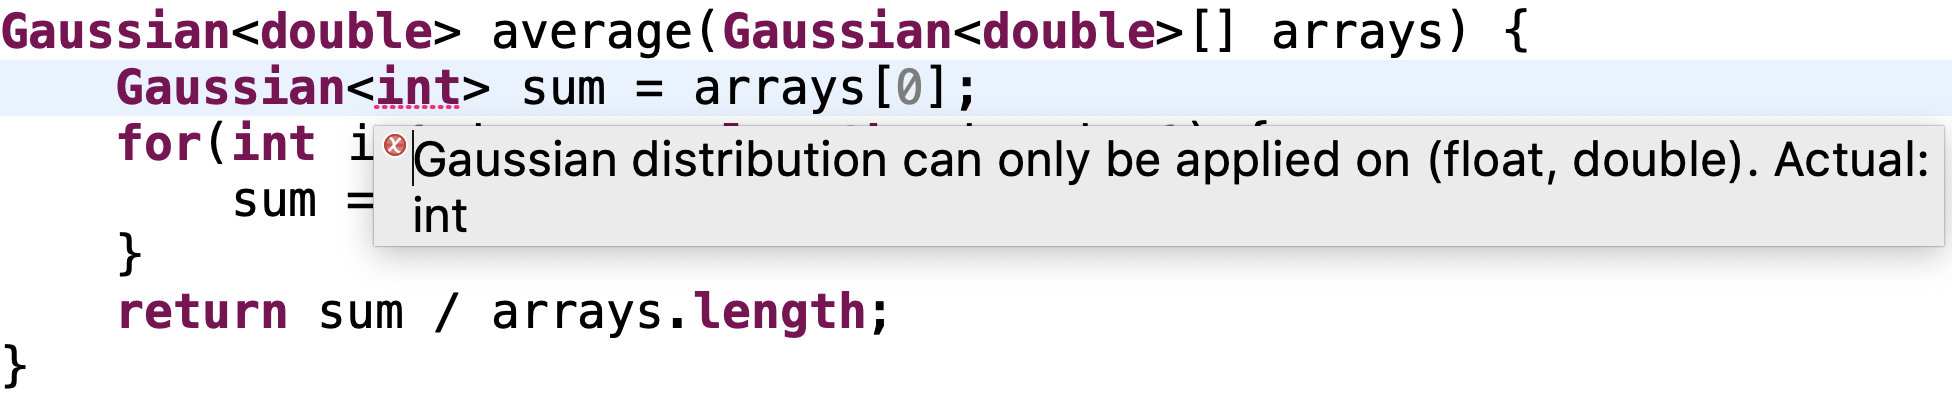
\includegraphics[width=0.6\linewidth]{img/motivation/aintea-overview}
%	\caption{Overview of the language proposed, \languageName{}}
%	\label{fig:motivation-aintea-overview}
%\end{figure}
\section{Validation}
\label{sec:tkm:validation}

To validate and evaluate our approach, we implemented a prototype publicly available online\footnote{https://github.com/lmouline/LDAS}.
This implementation leverages the GreyCat framework\footnote{https://github.com/datathings/greycat}, more precisely the modeling plugin, which allows designing a metamodel using a textual syntax.
Based on this specification, GreyCat generates a Java and a JavaScript API to create and manipulate models that conform to the predefined metamodel.
The GreyCat framework handles time as a built-in concept.
Additionally, it has a native support of a lazy loading mechanism and an advanced garbage collection.
This is achieved by dynamically loading and unloading model elements from the main memory when necessary.

The validation of our approach has been driven by the two research questions formulated in the introduction section:
\begin{itemize}
	\item How to diagnose the self-adaptation process?
	\item How to enable reasoning over unfinished actions and their expected effects?
\end{itemize}

To address the first one, we describe how one can use our approach to represent the knowledge an adaptation process for a smart grid system.
Then, we present a code to extract the circumstances and the goals of a decision.
For the second one, we present a scenario where a developer can use our approach to reason over unfinished actions and their expected effects.
The presented code shows how information can be extracted from our model to enable any reasoning algorithm.
Finally, we present performance evaluation to show the scalability of our approach.

\subsection{Diagnostic: implementation of the use case}
In what follows, we explain how a stakeholder, Morgan, can apply our approach to a smart grid system in order to, first, abstract adaptive system concepts, then, structure runtime data, and finally, query the model for diagnosis purpose.
The corresponding object model is depicted in Figure~\ref{fig:tkm:valid:diag}.
Due to space limitation, we only present an excerpt of the knowledge model.
An elaborate version is accessible in the tool repository.\looseness=-1

\paragraph{Abstracting the adaptive system}

At design time ($t_d$), either manually or using an automatic process, Morgan abstracts the different tactics and actions available in the adaptation process.
Among the different tactics that Morgan would like to model is  ``\textit{reduce amps limit}". 
It is composed of three actions: sending a request to the smart meter (\textit{askReduce}), checking if the new limit corresponds to the desired one (\textit{checkNewLimit}), and notifying the user by e-mail (\textit{notifyUser}). 
Morgan assumes that the \textit{askReduce} action impacts consumption data (\textit{csmpt}).
This tactic is triggered upon a query (\textit{tempQ}) that uses meter (\textit{mt}), consumption (\textit{csmpt}) and customer (\textit{cust}) data. The query implements the ``\textit{no overload}" goal: the system shall never have a cable overload. 
Figure~\ref{fig:tkm:valid:diag} depicts a flattened version of the temporal model representing these elements. The tag at upper-left corner of every object illustrates the creation timestamp. All the elements created at this stage are tagged with $t_d$.

\paragraph{Adding runtime information}
The adaptation process checks if the current system state fulfills the requirements by analyzing the context. To perform this, it executes the different temporal queries, including \textit{tempQ}.
For some reasons, the {tempQ} reveals that the current context does not respect the ``\textit{no overload}" goal. To adapt the smart grid system, the adaptation process decides to start the execution of the previously described tactic (\textit{exec1}) at $t_s$. As a result,  
a decision element is added to the model along with a relationship to the unsatisfied goal. In addition, this decision entails the planning of a tactic execution, manifested in the creation of the element \textit{exec1}and its subsequent actions (\textit{notifyU}, \textit{checkLmt}, and \textit{askRed}). At $t_s$, all the actions execution have an IDLE status and an expected start time. All the elements created at this stage are tagged with the $t_s$ timestamp in Figure~\ref{fig:tkm:valid:diag}.\looseness-1

At $t_{s+1}$, the planned tactic starts being executed by running the action \textit{askReduce}. The status of this action turns from \textit{IDLE} to \textit{RUNNING}. Later, at $t_{s+2}$, the execution of \textit{askReduce} finishes with a \textit{SUCCEED} status and triggers the execution of the actions \textit{notifyUser} and \textit{checkNewLimit} in parallel. The status of \textit{askReduce} changes to \textit{SUCCEED} while the status of \textit{notifyUser} and \textit{checkNewLimit} turns to \textit{RUNNING}.
The first action successfully ends at $t_{s+3}$ while the second ends at $t_{s+4}$. As all actions terminates with a \textit{SUCCEED} status at $t_{s+4}$, accordingly, the final status of the tactic is set \textit{SUCCEED} and the \textit{stop} attribute value is set to $t_{e}$.  

\begin{figure}
	\centering
	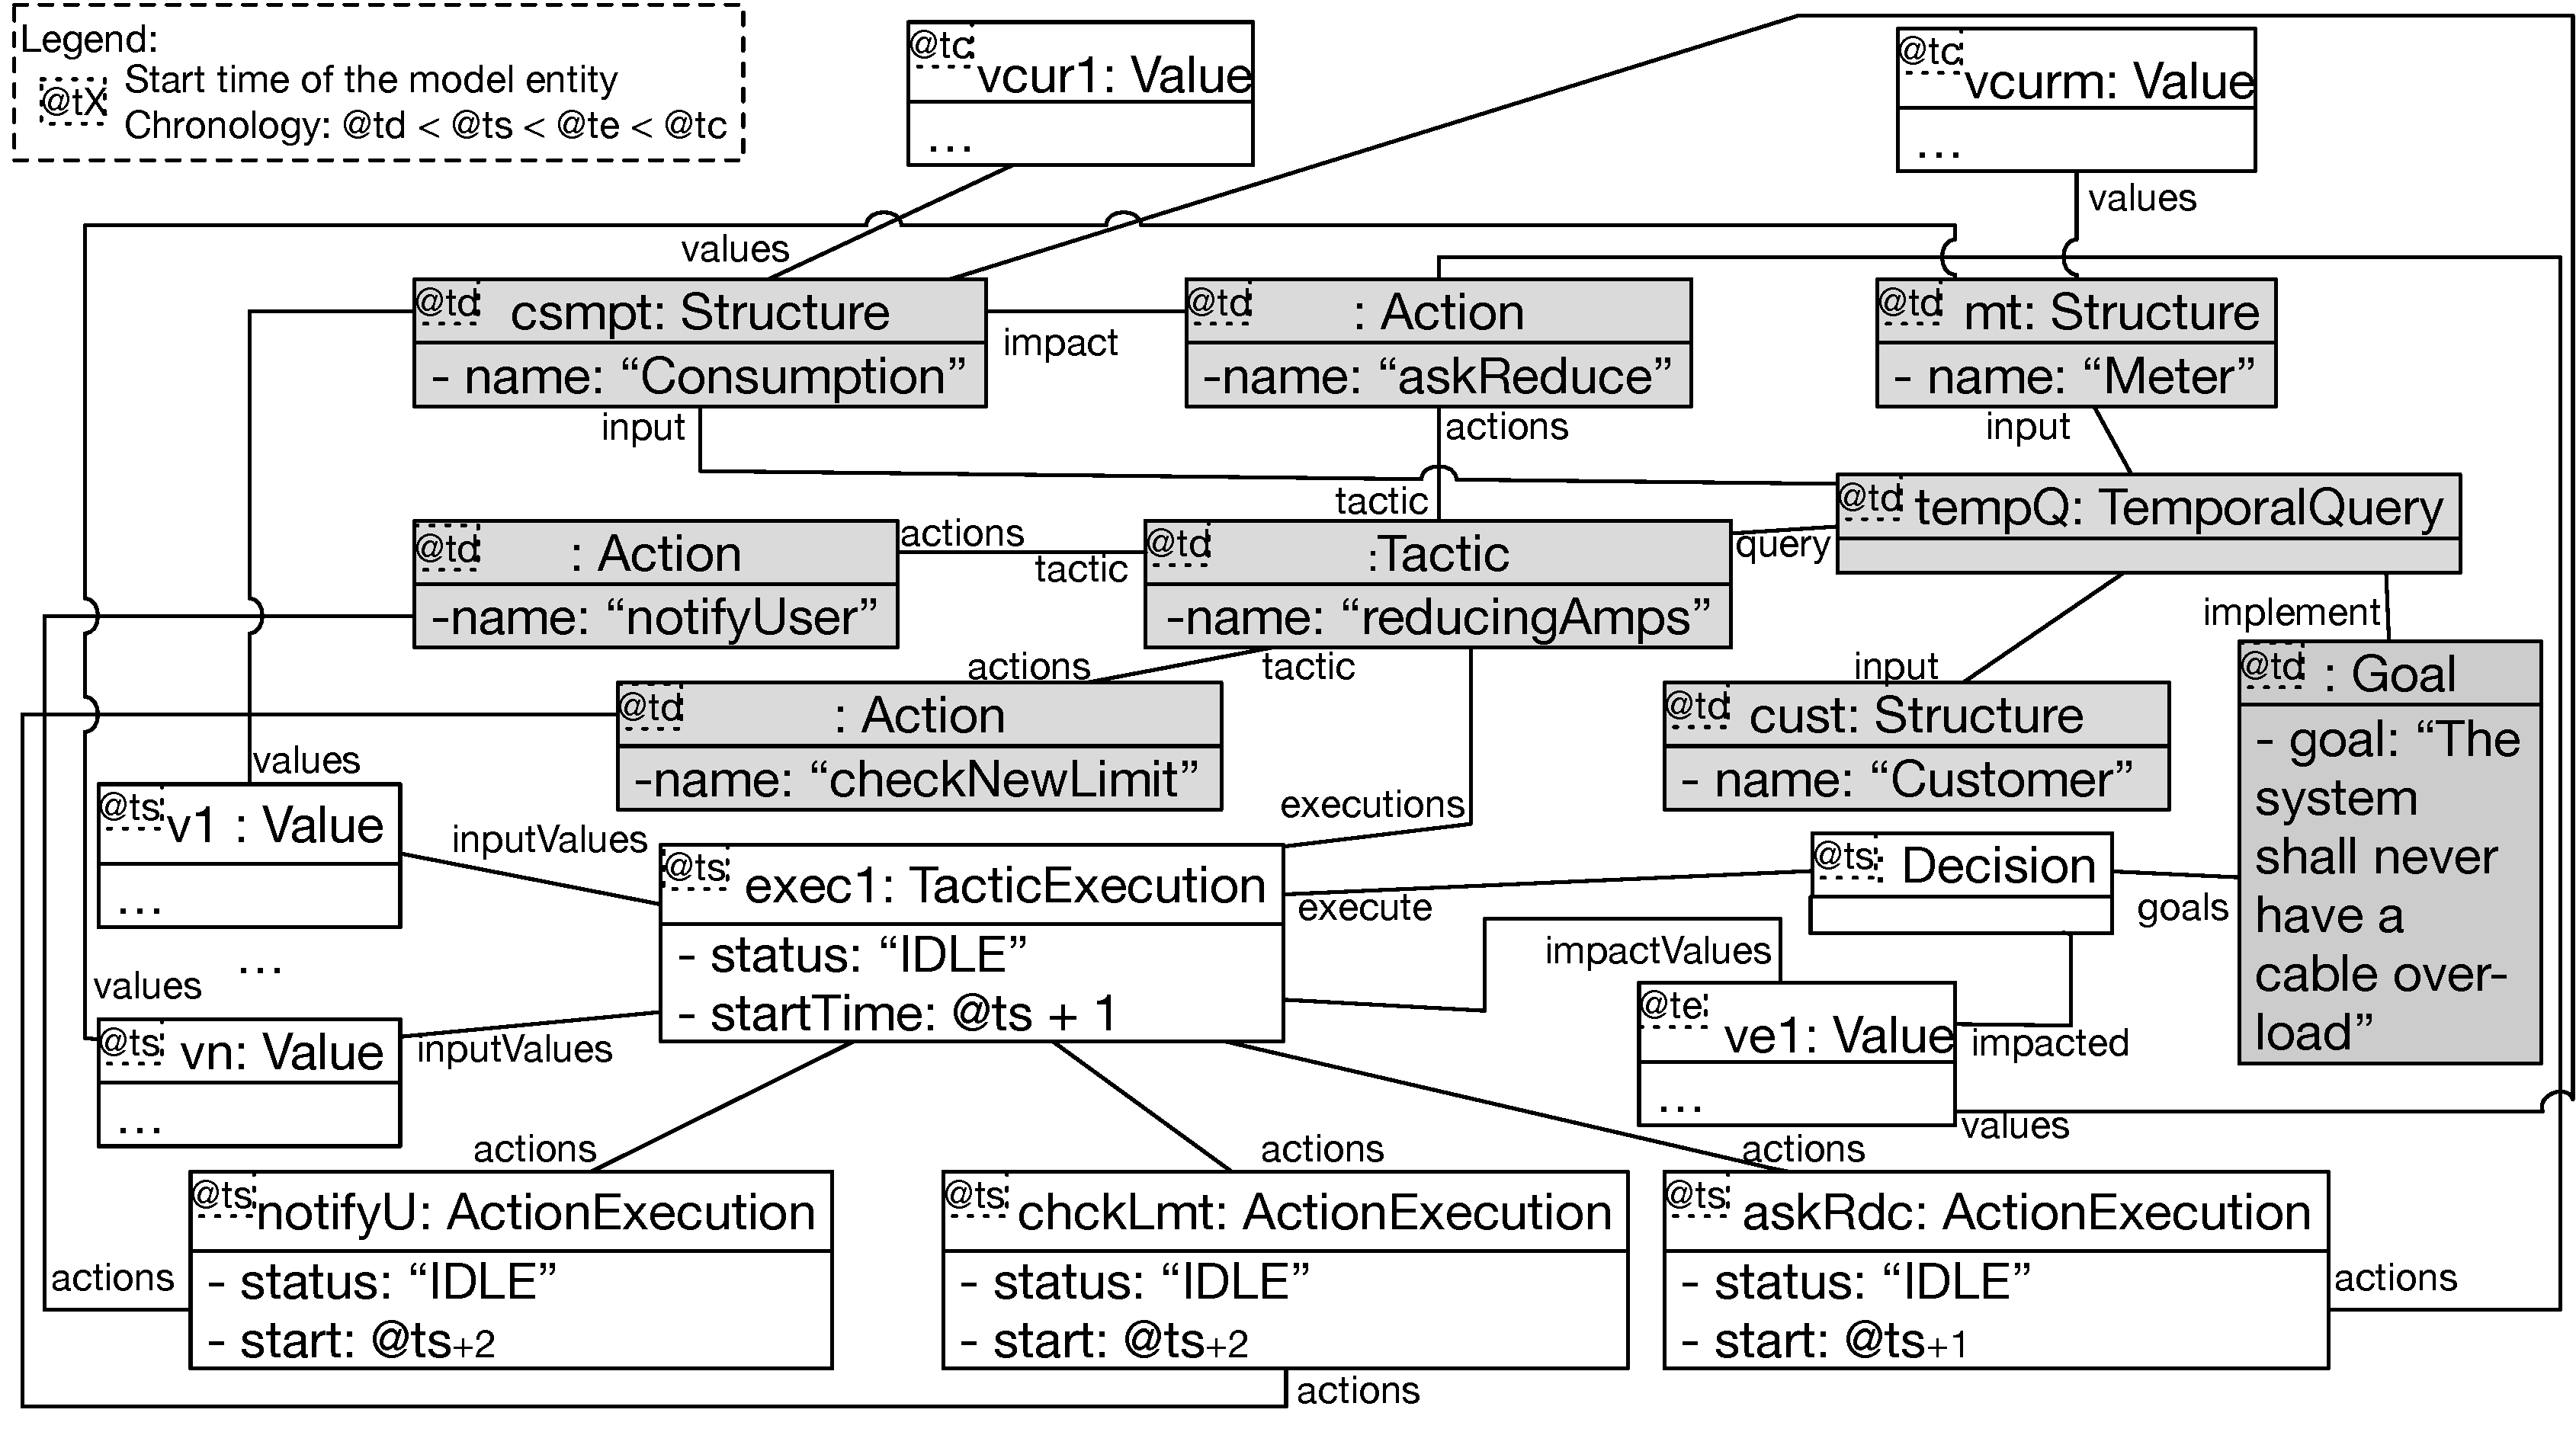
\includegraphics[width=\linewidth]{img/chapt-tkm/validation/action-om}
	\caption{Excerpt of the knowledge object model related to our smart grid example}
	\label{fig:tkm:valid:diag}
\end{figure}

\paragraph{Interactive diagnosis query}
After receiving incident reports concerning regular power cuts, and based on the aforementioned knowledge model, Morgan would be able to query the system's states and investigate why such incidents have occurred.
As described in Section~\ref{sec:example}, she/he will interactively diagnose the system by interrogating the context, the decisions made, and their circumstances.

The first function, depicted in Listing~\ref{code:actions-to-goals}, allows  to navigate from the currently measured values (\textit{vcur1}) to the decision(s) made. The for-loop and the if-condition are responsible for resolving the measured data for the past two days. 
Past elements are accessed using the \textit{resolve} function that implements the $\mathcal{Z}^T$ relation (\cf Section~\ref{sec:formalism}).
After extracting the decisions leading to power cuts, Morgan carries on with the diagnosis by accessing the circumstances of this decision. The code to perform this task is depicted in Listing~\ref{code:actions-to-goals}, the second function (getCircumstances).
Note that the relationship \textit{Decision.input} is the aggregation of \textit{Decision.excecute.inputValues}.

\begin{lstlisting}[style=customc,caption=Get the goals used by the adaptation process from executed actions, label=code:actions-to-goals,basicstyle=\scriptsize]
// extracting the decisions
Decision[] impactedBy(Value v) {
  Decision[] respD
  for( Time t: v.modificationTimes() ):
    if (t >= v.startTime() - 2 day)
      Value resV = resolve(v,t)
    respD.addAll(from(resV).navigate(Value.impacted))
  return respD
}
// extracting the circumstances of the made decisions
Tuple<Value[], Goal[]> getCircumstance(Decision d) {
  Value[] resValues = from(d).navigate(Decision.input)
  Goal[] resGoals = from(d).navigate(Decision.goals)      
  return Tuple<>(resValues, resGoals)
} 
\end{lstlisting}

\subsection{Reasoning over unfinished actions and their expected effects}
By associating the action model to the knowledge model, we aim at enhancing adaptation process with new abilities to reason.
In this section, we present an example of a reasoning algorithm which consider the impacts of running actions.
This example is based on our use case (\cf Section~\ref{sec:intro:use-case}).

Let's imagine that the adaption process detects overloaded cables in the smart grid.
To fix this situation, it takes severals counter measures, among which there are fuse state modifications.
As detailed in Section~\ref{sec:tkm:intro:motiv}, this action is considered as delayed action.
Later, another incident is detected, for example a substation is being overloaded.
Before taking any actions, the adaption process can, thanks to our solution, verify if the running actions will be sufficient to solve this new incidents.
If not, it can either take additional actions or replan the running one.
The algorithm to reschedule current actions or to compute additional actions is out of scope of this thesis.
Here, we present the code to extract required information from our model.

Checking if the running actions will be sufficient to solve all current issues can also be thought as: will the issue remain with the new context, \ie after each actions have been executed.
In our case, it is like verifying if the second overload will still remain with the new topology, which is coming.
The adaptation process therefore needs to extract the context in the future.
To do so, the adaptation process should know the latest timepoint at which the impact will be measured.
Listing~\ref{code:tkm:valid:latest-impact} shows the code to get this timepoint.
Running, idle and finished actions are accessed thanks to the the two first nested loops with the if-condition.
We consider that failed and canceled actions have no effects.
As finished actions may still have effects, we also consider them.
Then we navigate through all impacted values to get their start time, \ie the beginning of their validity period ($V^T$ relation, \cf Section~\ref{sec:tkm:k-formalism:formalism}).
Doing so, we are sure to get the latest timepoint at which an impact will be measurable.

\begin{lstlisting}[style=customc, caption=Get latest timepoint at which the impact will be measured, label=code:tkm:valid:latest-impact,basicstyle=\scriptsize]
Time latestImpact(Knowledge k) {
  Time latestTime = CURRENT_TIME
  
  for(Decision d: from(k).navigate(decisions))
    for(TacticExecution te: from(d).navigate(execute))
      if(te.status == "RUNNING" || te.status == "IDLE" || te.status == "SUCCEED")
        for(Value v: from(te).navigate(impactedValues))
          if(v.startTime() > latestTime)
            latestTime = v.startTime()
            
  return latestTime
}	
\end{lstlisting}

Using this timepoint, then the adaption process can then compute how the grid should be after the actions have been executed.
If the system has no prediction mechanism, then the adaption process can verify how the power will be balance over the new topology.
Otherwise, it can use this prediction feature to compute the expected loads with the coming topology.
Using these information, it can verify if all current incidents will be solved by the ongoing actions or not.
If not, it may take additional actions or reschedule them.

Listing~\ref{code:tkm:valid:extract-act} depicts the code to extract all running actions.
The nested loops allow accessing to all executions made by decision.
Then, we filter only those with the \textquote{RUNNING} status.
The resulting collection should then be given to the scheduling algorithm, which will decide if a rescheduling is possible and how. 

 
\begin{lstlisting}[style=customc, caption=Extract ongoing actions and their effects, label=code:tkm:valid:extract-act,basicstyle=\scriptsize]
TacticExecution[] runningActions(Knowledge k) {
  TacticExecution[] resA
  for(Decision d: k.decisions) {
    for(TacticExecution te: d.execute) {
      if(te.status == Status.RUNNING) {
        resA.add(te)
      }
    }
  }
  return resA
}
\end{lstlisting}

Using our model, developers have to solution to model a rescheduling operation.
Either they modify the actions, which may delete the history of the previous decision, or they mark all running and idle actions as \textquote{CANCELLED} and create a new decision, with new actions, which update the circumstances and re-use the same requirements.

\subsection{Performance evaluation}
GreyCat stores temporal graph elements in several key/value maps. Thus, the complexity of accessing a graph element is linear and depends on the size of the graph. 
Note that in our experimentation we evaluate only the execution performance of diagnosis algorithms. For more information on I/O performance in GreyCat, please refer to the original work by Hartmann \etal~\cite{DBLP:conf/seke/0001FJRT17, DBLP:phd/basesearch/Hartmann16}.

\begin{lstlisting}[style=customc,caption=Traversal used during the experimentations,label=code:traversal-used,basicstyle=\scriptsize]
  MATCH (input)-[*4]->(output)
  WHERE input.id IN [randomly generated set]
  RETURN output
  LIMIT O
\end{lstlisting}

We consider a diagnosis algorithm to be a graph navigation from a set of nodes (input) to another set of nodes (output).
Unlike typical graph algorithms, diagnosis algorithms are simple graph traversals and do not involve complex computations at the node level. Hence, we believe that three parameters can impact their performance (memory and/or CPU): the global size of the graph, the size of the input, and the number of traversed elements.
In our evaluation, we altered these parameters and report on the behavior of the main memory and the execution time. The code of our evaluation is publicly available online\footnote{https://bitbucket.org/ludovicpapers/icac18-eval}.
All experiments reporting on memory consumption were executed 20 times after one warm-up round. Whilst, execution time experiments were run 100 times after 20 warm-up rounds.
The presented results correspond to the mean of all the iterations.
We randomly generate graph with sizes (\textit{N}) ranging from 1\,000 to 2\,000\,000. 
At every execution iteration, we follow these steps: (1) in a graph with size \textit{N}, we randomly select a set of \textit{I} input nodes, (2) then traverse \textit{M} nodes in the graph, (3) and  we collect  the first \textit{O} nodes that are at four hops from the input element. Listing~\ref{code:traversal-used} describes the behavior of the traversal using Cypher, a well-known graph traversal language.

We executed our experimentation on a MacBook Pro with an Intel Core i7 processor (2.6 GHz, 4 cores, 16GB main memory (RAM), macOS High Sierra version 10.13.2). We used the Oracle JDK version 1.8.0\_65.

\paragraph{How performance is influenced by the graph size \textit{N}?}
This experimentation aims at showing the impact of the graph size (\textit{N}) on memory and execution time while performing common diagnosis routines.
We fix the size of \textit{I} to 10. To assure that the behavior of our traversals is the same, we use a seed value to select the starting input elements. We stop the algorithm when we reach 10 elements.
Results are depicted in Figure~\ref{fig:exp1}.

As we can notice, the graph size does not have a significant impact on the execution time of diagnosis algorithms.
For graphs with up to 2,000,000 elements, execution time remains between 2 ms and four 4 ms. We can also notice that the memory consumption insignificantly increases.
Thanks to the implementation of a lazy loading and a garbage collection strategy by GreyCat, the graph size does not influence memory or execution time performance. The increase in memory consumption can be due to the internal indexes or stores that grow with the graph size.

\begin{figure}
	\centering
	\subfloat[Execution time evolution] {
			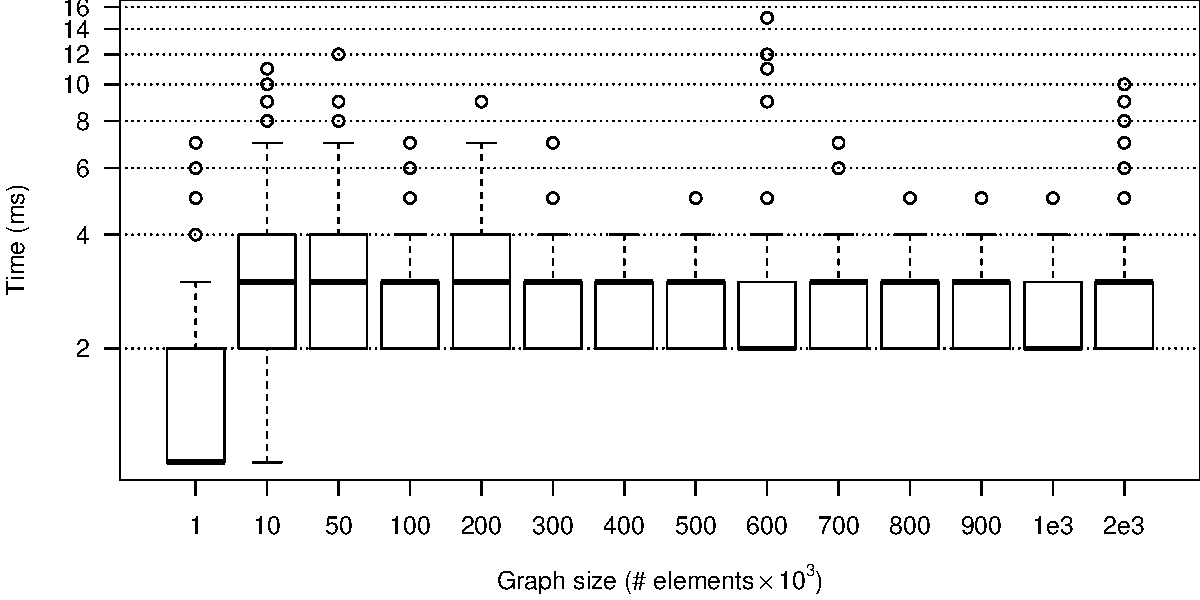
\includegraphics[width=0.85\linewidth]{img/chapt-tkm/validation/exp1-exec-log}
			\label{fig:exp1-exec}
	}
	\hfil
	\subfloat[Memory evolution] {
			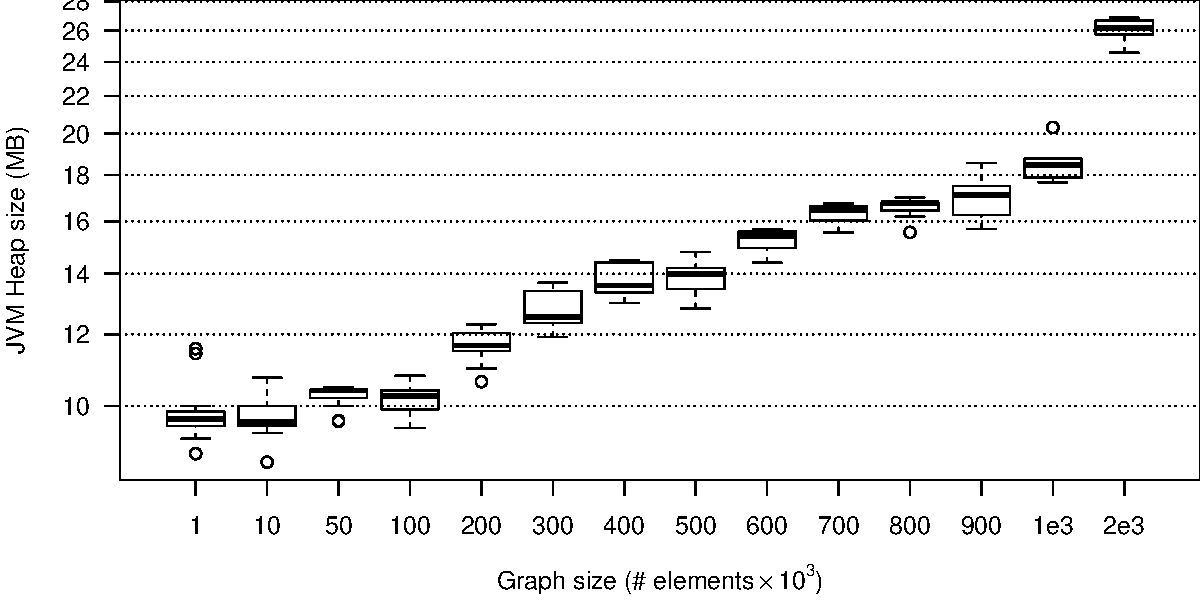
\includegraphics[width=0.85\linewidth]{img/chapt-tkm/validation/exp1-mem-log}
			\label{fig:exp1-mem}
		}	
	\caption{Experimentation results when the knowledge based size increases}
	\label{fig:exp1}
\end{figure}

\paragraph{How performance is influenced by the input size (I)?}
The second experiment aims to show the impact of the input size (I) on the execution of diagnosis algorithms. We fix the size of \textit{N} to 500\,000 and we variate \textit{I} from 1\,000 nodes to 100\,000, \ie from 0.2\% to 20\% of the graph size. 
The results are depicted in Figure~\ref{fig:exp-res} (straight lines).

Unlike to the previous experiment, we notice that the input size (\textit{I}) impacts the performance, both in terms of memory consumption and execution time. This is because our framework keeps in memory all the traversed elements, namely the input elements.
The increase in memory consumption follows a linear trend with regards to \textit{N}. As it can be noticed, it reaches 2GB for \textit{I}=100\,000. The execution time also shows a similar curve, while the query response time takes around than around 60ms to run for \textit{I}=1\,000, it takes a bit more than 4 seconds to finish for \textit{I}=100\,000. Nonetheless, these results remain very acceptable for diagnosis purposes. 

\paragraph{How performance is influenced by the number of traversed elements (M)?}%
For the last experiment, we aim to highlight the impact of the number of traversed elements (\textit{M}). For this, we fix \textit{I} and \textit{O} to 1, and randomly generate a graph with sizes ranging from $1\,000$ to $100\,000$. Our algorithm navigates the whole model (\textit{M}=\textit{N}).
We depict the results in Figure~\ref{fig:exp-res} (dashed curve).
As we can notice, the memory consumption increases in a quasi-linear way. The memory footprint to traverse \textit{M} = 100\,000 elements is around 0.9GB. The progress of the execution time curve behaves similarly, in a quasi-linear way. Finally, the execution time of a full traversal over the biggest graph takes less than 2.5 seconds. 

\begin{figure}
	\centering
	\subfloat[Evolution of the execution time]{
		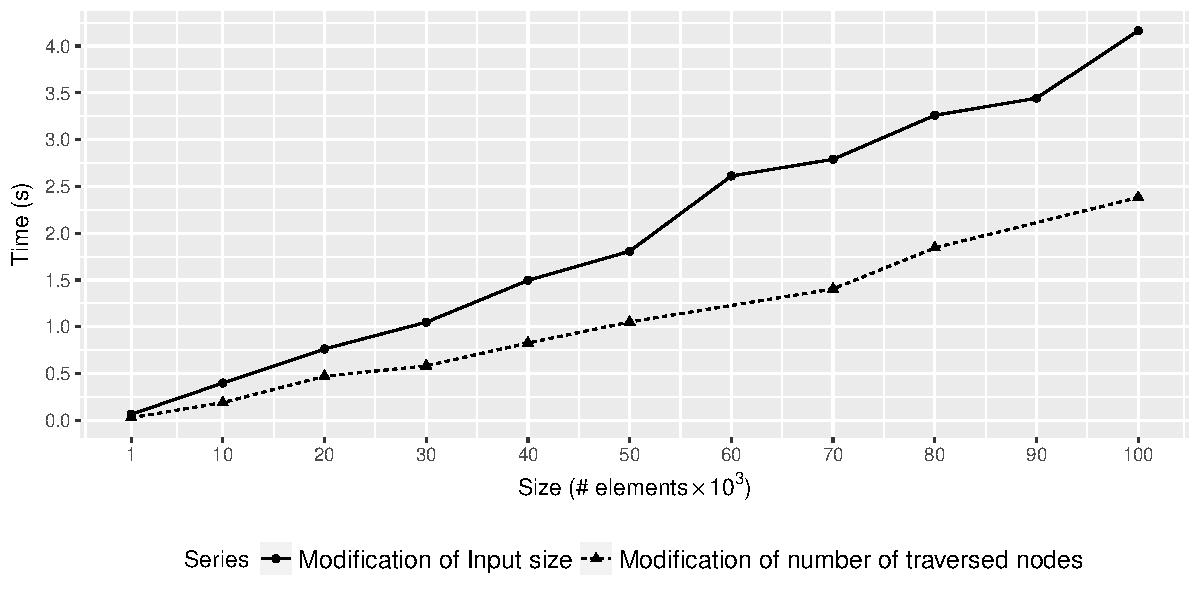
\includegraphics[width=0.9\linewidth]{img/chapt-tkm/validation/exp-exec}
		\label{fig:exp-exec}
	}
	\hfil
	\centering
	\subfloat[Evolution of the memory consumption]{
		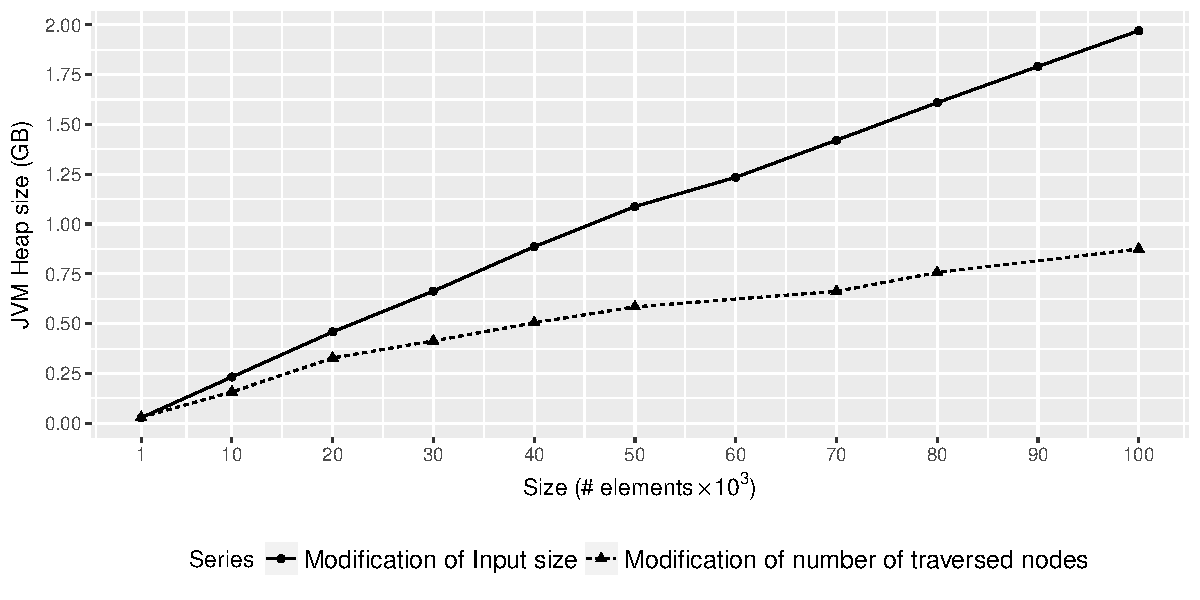
\includegraphics[width=0.9\linewidth]{img/chapt-tkm/validation/exp-mem}
		\label{fig:exp-mem}
	}
\caption{Results of experiments when the number of traversed or input elements  increases}
\label{fig:exp-res}
\end{figure}

\subsection{Discussion}
By linking context, actions, and requirements using decisions, data extraction for explanation or fault localization can be achieved by performing common temporal graph traversal operations.
In the detailed example, we show how a stakeholder could use our approach to define the different elements required by such systems, to structure runtime data, finally, to diagnose the behavior of adaptation processes. 

Our implementation allows to dynamically load and release nodes during the execution of a graph traversal. Using this feature, only the needed elements are kept in the main memory.  Hence, we can perform interactive diagnosis routines on large graphs with an acceptable memory footprint. 
However, the performance of our solution, in terms of memory and execution time, is restricted by the number of traversed elements and the number of input elements.
Indeed, as shown in our experimentation, both the execution time and the memory consumption grow linearly.

As described in~\cite{DBLP:conf/smartgridcomm/0001FKTPTR14}, the smart grid in Luxembourg is composed of 1 central system, 3 data concentrators and 227 meters.
The network is thus composed of 231 elements.
Each meter sends the consumption value every 15 min, being 908 every hours.
Plus, there is from 0 to 273 topology modifications in the network.
In total, the system generates from 908 to 1,181 new values every hour.
If we consider that we have one model element per smart grid entity and one model element per new value, 100,000 model elements correspond thus from $((100,000 - 231) * 1H ) / 1,181 = 84,5H$ ($\sim$ 3,5 days) to $((100,000 - 231) * 1H ) / 908 = 109,9H$ ($\sim$ 4,6 days) of data. In other word, our approach can efficiently interrogate up to $\sim$5 days history data in 2.4s.


\section{Conclusion}
\label{sec:sota:conclusion}